\documentclass[main.tex]{subfiles}
\begin{document}
\section{Approximation and Taylor polynomial}

Some problems are too difficult to solve exactly, but can be approximated close to a point with great accuracy by a simply mathematical tool. We have already seen an approximation in equation \ref{linapprox}, i have taken the liberty to change the names of the points on the x-axis in the equation: 
\begin{equation}
f(x) \approx L(x) = f(a) + f'(a)(x-a)
\end{equation}
This equation states that the approximated value of the function at the point $x$ on the x-axis can be calculated by the function value at the point $a$ plus the derivative at $a$ multiplied by the length between the point $x$ and $a$ on the x-axis. In other words using differentials, we can see how the function behaves close to a point. The above function is the definition for the \textbf{linearization} of the function $f$ about $a$ is the function $L$, where $f(x) \approx L(x)$ provides linear approximations for the values of the function near $a$. The error of the approximation is defined by

\begin{align}
\mathtt{error} \; =& \; \mathtt{true \; value} - \mathtt{approximate \; value} \\
E(x) =& f(x) - L(x) = f(x) - f(a) - f'(a)(x-a)
\end{align}

\begin{figure}
\begin{center}
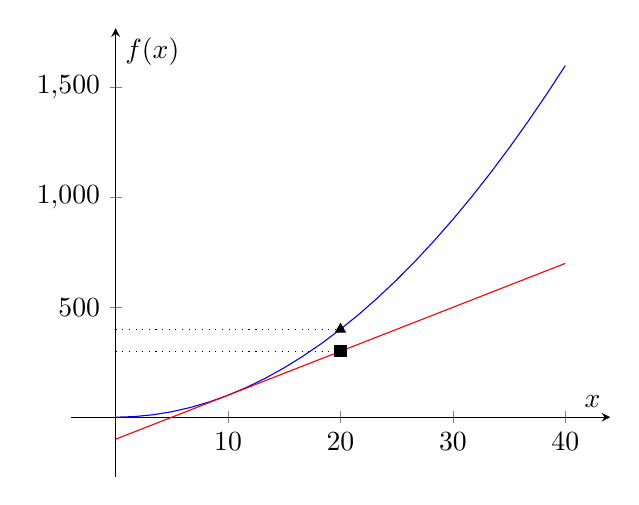
\begin{tikzpicture}
\begin{axis}[axis lines=middle,xlabel=$x$,ylabel=$f(x)$,enlargelimits]
\addplot[domain= 0:40, blue]{x^2};
\addplot[domain= 0:40, red]{20*x-100};
\addplot[domain= 0:20, dotted]{400};
\addplot[domain= 0:20, dotted]{300};
\addplot[
scatter,
only marks,
point meta=explicit symbolic,
scatter/classes={b={mark=triangle*,draw=black},%
c={mark=square*,black}},
]
table[meta=label] {
      x y label
      20 400 b
      20 300 c
      };
\end{axis}
\end{tikzpicture}
\caption{The blue graph is $f(x)=x^2$ and the red $L(x)=20x-100$, where the red graph is the linerization $L(x)$ of $f(x)=x^2$ around $a=10$. The point $(20,f(20))$ is marked with a black triangle and the point $(20,L(20))$ is marked with a black square. As seen, there is a difference between $f(20)$ and $L(20)$, this difference is called the error.}
\end{center}
\end{figure}

But how can we approximate the behaviour the function better and with less error. We use the Taylor polynomial to approximate the function. The linearization is a polynomial of degree $1$. The Taylor polynomial lets us approximate the function using higher degree polynomials about a point $a$. The Taylor polynomial is defined by:

\begin{equation}
P_n(x) = f(a) + \frac{f'(a)}{1!}(x-a) + \frac{f''(a)}{2!}(x-a)^2 + \frac{f'''(a)}{3!}(x-a)^3 + ... + \frac{f^{(n)}(a)}{n!}(x-a)^n,
\end{equation}      

The factorial $n!$ is defined as $n \cdot (n-1) \cdot (n-2) \cdot ... \cdot 1$, $f'(a)$ is the first derivative at $a$, $f''(a)$ is the second derivative (differentiate $f'(a)$ again), $f^{(n)}$ is the n th derivative. Let delve into this new mathematical tool through an example.

\begin{example}
Lets find the second order Taylor polynomial of the function $f(x) = \sqrt{x}$ about $a=25$. Lets first write the the second order Taylor polynomial $P_2(x)$ mathematically:

\begin{equation}
P_2(x) = f(a) + \frac{f'(a)}{1!}(x-a) + \frac{f''(a)}{2!}(x-a)^2
\end{equation}
We stopped at the third term because we have the second order derivative of $f(a)$. If we wanted the third order Taylor polynomials we would have to go to the fourth term were we have the third order derivative. The first derivative of $f(x)$ is $f'(x)=\frac{1}{2}x^{-1/2}$ and the second derivative is $f''(x) = -\frac{1}{4}x^{-3/2}$. Now lets slowly begin to place the derivatives in the second order Taylor polynomial and place $a=25$.

\begin{align}
P_2(x) =& f(25) +f'(25)(x-25) + \frac{f''(25)}{2}(x-25)^2\\
=& \sqrt{25} + \frac{1}{2}(25)^{-1/2}(x-25) -\frac{1}{8}x^{-3/2}(x-25)^2 \\
=& 5 + \frac{1}{10}(x-25) - \frac{1}{1000}(x-25)^2 \\
=& -\frac{x^2}{1000} + \frac{3}{20}x + \frac{15}{8}
\end{align}  
So what do we have here? We have a second order polynomial that approximates the function values of $f(x)=\sqrt{x}$ around the point $a=25$. Lets see what function value we get out in both for $x = 26$:

\begin{equation}
f(26) = \sqrt{26} = 5.099
\end{equation}

\begin{equation}
P_2(26) = -\frac{26^2}{1000} + \frac{3}{20} \cdot 26 + \frac{15}{8} = 5.099
\end{equation}

So the second order polynomial approximates the function value at $x = 26$ to four decimal places exactly. What if we want to approximate the function value at $x=35$:

\begin{equation}
f(35) = \sqrt{35} = 5.9161
\end{equation}

\begin{equation}
P_2(35) = -\frac{35^2}{1000} + \frac{3}{20}35 + \frac{15}{8} = 5.9000
\end{equation}

We can see that the second order polynomial is quite close to the function value. 

\begin{figure}
\begin{center}
\begin{minipage}[t]{0.45\linewidth}
\begin{tikzpicture}
\begin{axis}[axis lines=middle,xlabel=$x$,ylabel=$f(x)$,enlargelimits]
\addplot[domain=0:40, blue] {sqrt(x)};
\addplot[domain=0:40, red] {-x^2/1000 + 3*x/20 + 15/8};
\end{axis}
\end{tikzpicture}
\caption{The blue graph is $f(x) = \sqrt x$ and the red $-\frac{x^2}{1000} + \frac{3}{20}x + \frac{15}{8}$}
\end{minipage}
\quad
\begin{minipage}[t]{0.45\linewidth}
\begin{tikzpicture}
\begin{axis}[axis lines=middle,xlabel=$x$,ylabel=$f(x)$,enlargelimits]
\addplot[domain=0:40, red] {sqrt(x)-(-x^2/1000 + 3*x/20 + 15/8)};
\end{axis}
\end{tikzpicture}
\caption{$E(x) = \sqrt x - (-\frac{x^2}{1000} + \frac{3}{20}x + \frac{15}{8}) $}
\end{minipage}
\end{center}
\end{figure}
 
\end{example}

\begin{example}
Let us now look at the function $f(x)=\sin(x)$ and find the fifth order Taylor polynomial around $a=0$.
\begin{align}
P_5(x) =& f(0) + \frac{f'(0)}{1!}(x-0) + \frac{f''(0)}{2!}(x-0)^2 + \frac{f'''(0)}{3!}(x-0)^3 + \frac{f''''(0)}{4!}(x-0)^4 + \frac{f'''''(0)}{5!}(x-0)^5 \\
=& \sin(0) + \cos(0)x - \frac{\sin(0)}{2}x^2-\frac{\cos(0)}{6}x^3+\frac{\sin(0)}{24}x^4+\frac{\cos(0)}{120}x^5 \\
=& 0 + x + -\frac{1}{6}x^3+0+\frac{1}{120}x^5
\end{align}

\begin{figure}
\begin{center}
\begin{minipage}[t]{0.45\linewidth}
\begin{tikzpicture}
\begin{axis}[axis lines=middle,xlabel=$x$,ylabel=$f(x)$,enlargelimits]
\addplot[domain =0:2, blue] {sin(deg(x))};
\addplot[domain =0:2, red] {x};
\end{axis}
\end{tikzpicture}
\caption{The blue graph represents $f(x) = \sin(x)$ and the red $f(x)= x$}
\end{minipage}
\quad
\begin{minipage}[t]{0.45\linewidth}
\begin{tikzpicture}
\begin{axis}[axis lines=middle,xlabel=$x$,ylabel=$f(x)$,enlargelimits]
\addplot[domain=0:2, red] {sin(deg(x))-x};
\end{axis}
\end{tikzpicture}
\caption{$E(x) = \sin(x)-x$}
\end{minipage}
\end{center}
\end{figure}

\end{example}
\end{document}